\documentclass[../../main/main.tex]{subfiles}
\graphicspath{{./figures/}}

\dominitoc
\faketableofcontents

\makeatletter
\renewcommand{\@chapapp}{Architecture de la mati\`ere -- chapitre}
\makeatother

% \toggletrue{student}
% \HideSolutionstrue
% \toggletrue{corrige}
% \renewcommand{\mycol}{black}
\renewcommand{\mycol}{gray}

\settasks{label=$\diamond$}

\begin{document}
\setcounter{chapter}{1}

\chapter{Propri\'et\'es physico-chimiques macroscopiques}

\vspace*{\fill}
% \vspace{-15pt}
\begin{prgm}
	\begin{tcb}*(ror)"know"{Savoirs}
		\begin{itemize}
			\item Interactions de \textsc{Van der Waals}. Liaison hydrogène ou
			      interaction par pont hydrogène.
			\item Grandeurs caractéristiques et propriétés de solvants moléculaires~:
			      moment dipolaire, permittivité relative, caractère protogène.
			\item Mise en solution d'une espèce chimique moléculaire ou ionique.
		\end{itemize}
	\end{tcb}
	\begin{tcb}*(ror)"how"{Savoir-faire}
		\begin{itemize}
			\item Citer les ordres de grandeur énergétiques des interactions de
			      \textsc{Van der Waals} et de liaisons hydrogène.
			\item Interpréter l'évolution de températures de changement d'état de
			      corps purs moléculaires à l'aide de l'existence d'interactions de
			      \textsc{Van der Waals} ou par pont hydrogène.
			\item Associer une propriété d'un solvant moléculaire à une ou des
			      grandeurs caractéristiques.
			\item Interpréter la miscibilité ou la non-miscibilité de deux solvants.
			\item Interpréter la solubilité d'une espèce chimique moléculaire ou
			      ionique.
		\end{itemize}
	\end{tcb}
\end{prgm}

% \vspace*{\fill}

% \newpage

\vspace*{\fill}
\minitoc
\vspace*{\fill}

\newpage

\vspace*{\fill}
\begin{boxes}
	\begin{tcb}(defi)<lftt>{Liste des définitions}
		\tcblistof[\paragraph*]{defi}{\hspace*{6pt}}
	\end{tcb}
	% \begin{tcb}(rapp)<lftt>{Liste des rappels}
	% 	\tcblistof[\paragraph*]{rapp}{\hspace*{6pt}}
	% \end{tcb}
	% \begin{tcb}(prop)<lftt>{Liste des propriétés}
	% 	\tcblistof[\paragraph*]{prop}{\hspace*{6pt}}
	% \end{tcb}
	% \begin{tcb}(coro)<lftt>{Liste des corollaires}
	% 	\tcblistof[\paragraph*]{coro}{\hspace*{6pt}}
	% \end{tcb}
	% \begin{tcb}(demo)<lftt>{Liste des démonstrations}
	% 	\tcblistof[\paragraph*]{demo}{\hspace*{6pt}}
	% \end{tcb}
	% \begin{tcb}(inte)<lftt>{Liste des interprétations}
	% 	\tcblistof[\paragraph*]{inte}{\hspace*{6pt}}
	% \end{tcb}
	% \begin{tcb}(tool)<lftt>{Liste des outils}
	% 	\tcblistof[\paragraph*]{tool}{\hspace*{6pt}}
	% \end{tcb}
	% \begin{tcb}(nota)<lftt>{Liste des notations}
	% 	\tcblistof[\paragraph*]{nota}{\hspace*{6pt}}
	% \end{tcb}
	% \begin{tcb}(appl)<lftt>{Liste des applications}
	% 	\tcblistof[\paragraph*]{appl}{\hspace*{6pt}}
	% \end{tcb}
	\begin{tcb}(rema)<lftt>{Liste des remarques}
		\tcblistof[\paragraph*]{rema}{\hspace*{6pt}}
	\end{tcb}
	\begin{tcb}(exem)<lftt>{Liste des exemples}
		\tcblistof[\paragraph*]{exem}{\hspace*{6pt}}
	\end{tcb}
	\begin{tcb}(ror)<lftt>{Liste des points importants}
		\tcblistof[\paragraph*]{ror}{\hspace*{6pt}}
	\end{tcb}
	% \begin{tcb}(impo)<lftt>{Liste des erreurs communes}
	% 	\tcblistof[\paragraph*]{impo}{\hspace*{6pt}}
	% \end{tcb}
\end{boxes}
\vspace*{\fill}
\newpage

À température ambiante, le dichlore est gazeux, le dibrome est liquide et le
diiode solide~: il y a donc des interactions qui expliquent la cohésion des
molécules entre elles malgré l'agitation thermique. Le but de ce chapitre est de
lister les forces intermoléculaires pour comprendre la cohésion de la matière.

\section{Interactions de \textsc{Van der Waals}}

\begin{tcb*}(defi){Interactions de \textsc{Van der Waals}}
	Les interactions de \textsc{Van der Waals} regroupent trois types d'interactions
	électrostatiques \textbf{attractives et additives} entre les molécules. Toutes
	ces forces sont donc attractives, et diminiuent très rapidement avec la distance
	entre les molécules. L'énergie potentielle d'interaction entre deux molécules
	séparées d'une distance $d$ est de la forme
	\psw{
		\[\boxed{\Ec_{p,VdW} = -\frac{\cte}{d^6}}\]
	}
	\vspace{-15pt}
\end{tcb*}

\subsection{Interaction dipôle/charge}

Physiquement, un moment dipolaire traduit une dissymétrie de charges entre deux
«~extrémités~» d'une molécule. Cette dissymétrie rend la molécule capable
d'interagir avec d'autres charges, voir Figure~\ref{fig:dipq}~: très
schématiquement, une charge positive placée à proximité de la molécule est
globalement attirée par l'extrémité chargée $\de-$ et globalement repoussée par
l'extrémité chargée $\de+$. C'est bien sûr le contraire pour une charge
négative.

\begin{figure}[H]
	\centering
	\sswitch{
		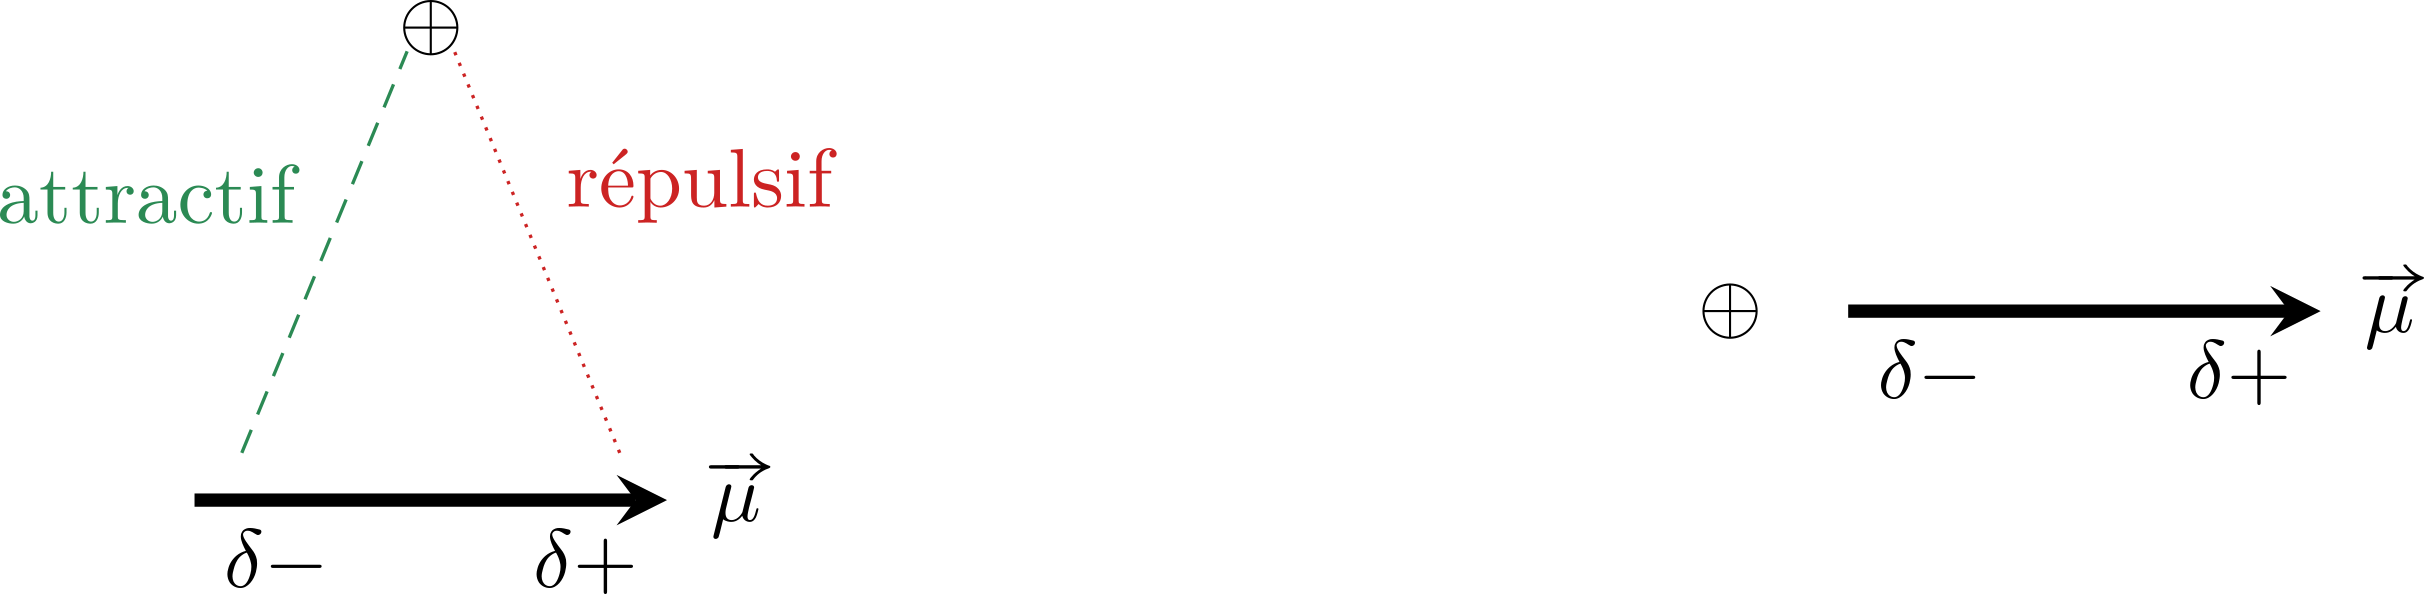
\includegraphics[scale=1, draft=true]{dipq}
	}{
		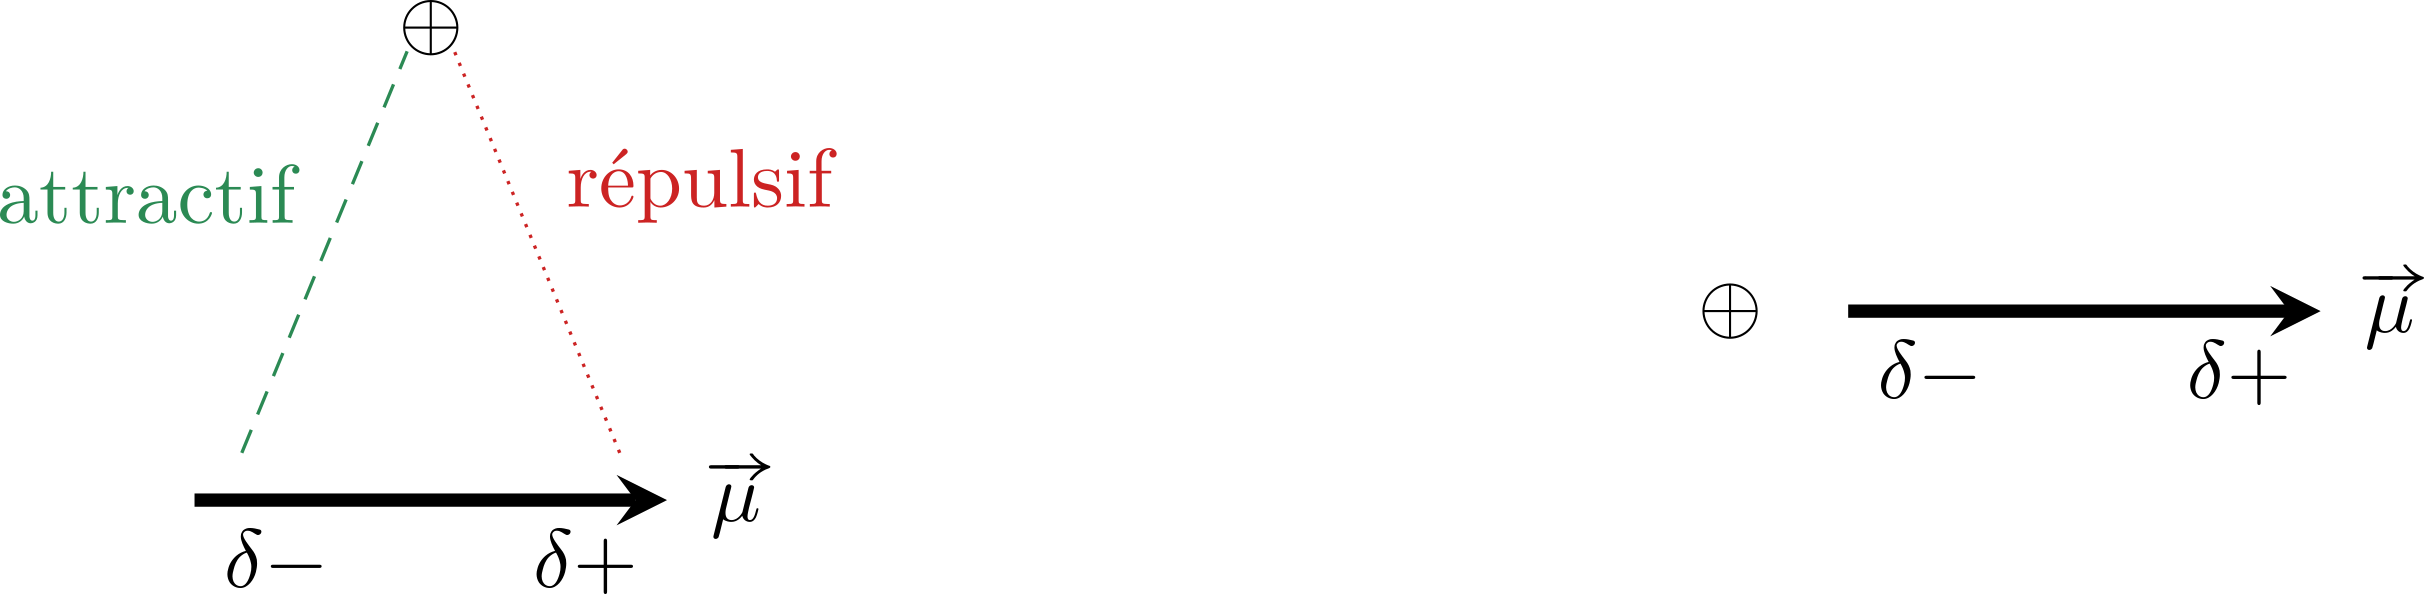
\includegraphics[scale=1]{dipq}
	}
	\caption{Interaction électrostatique entre un dipôle et une charge.}
	\label{fig:dipq}
\end{figure}

\subsection{Interaction de \textsc{Keesom}~: permanent/permanent}

Le mécanisme discuté précédemment se généralise aux cas d'une interaction entre
deux dipôles, voir Figure~\ref{fig:keesom}~: la charge $\de-$ du dipôle 2 tend à
se placer derrière la charge $\de+$ du dipôle 1, et réciproquement. On peut
alors montrer que la position d'équilibre du dipôle 2 est celle où il est aligné
avec le dipôle 1.

\begin{figure}[H]
	\centering
	\sswitch{
		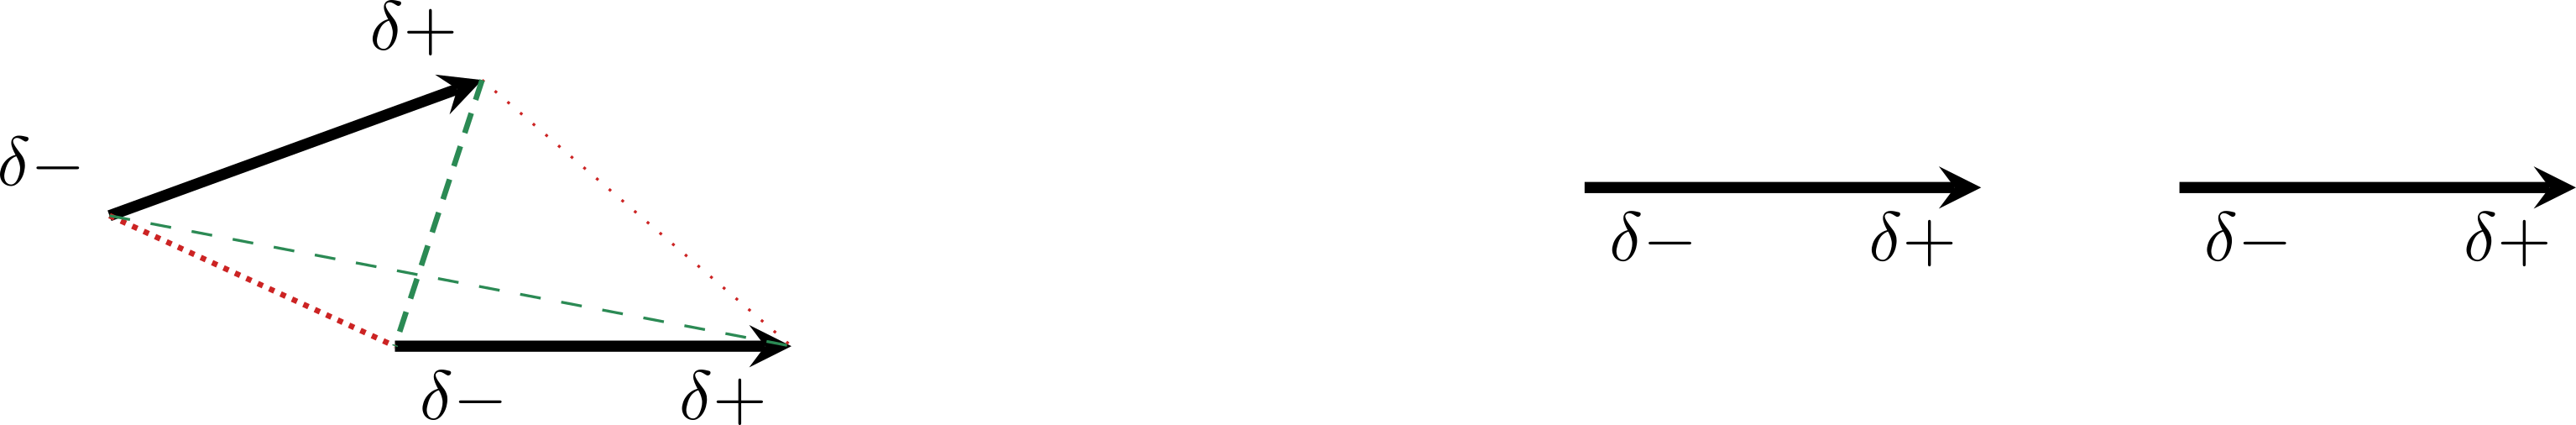
\includegraphics[scale=1, draft=true]{keesom}
	}{
		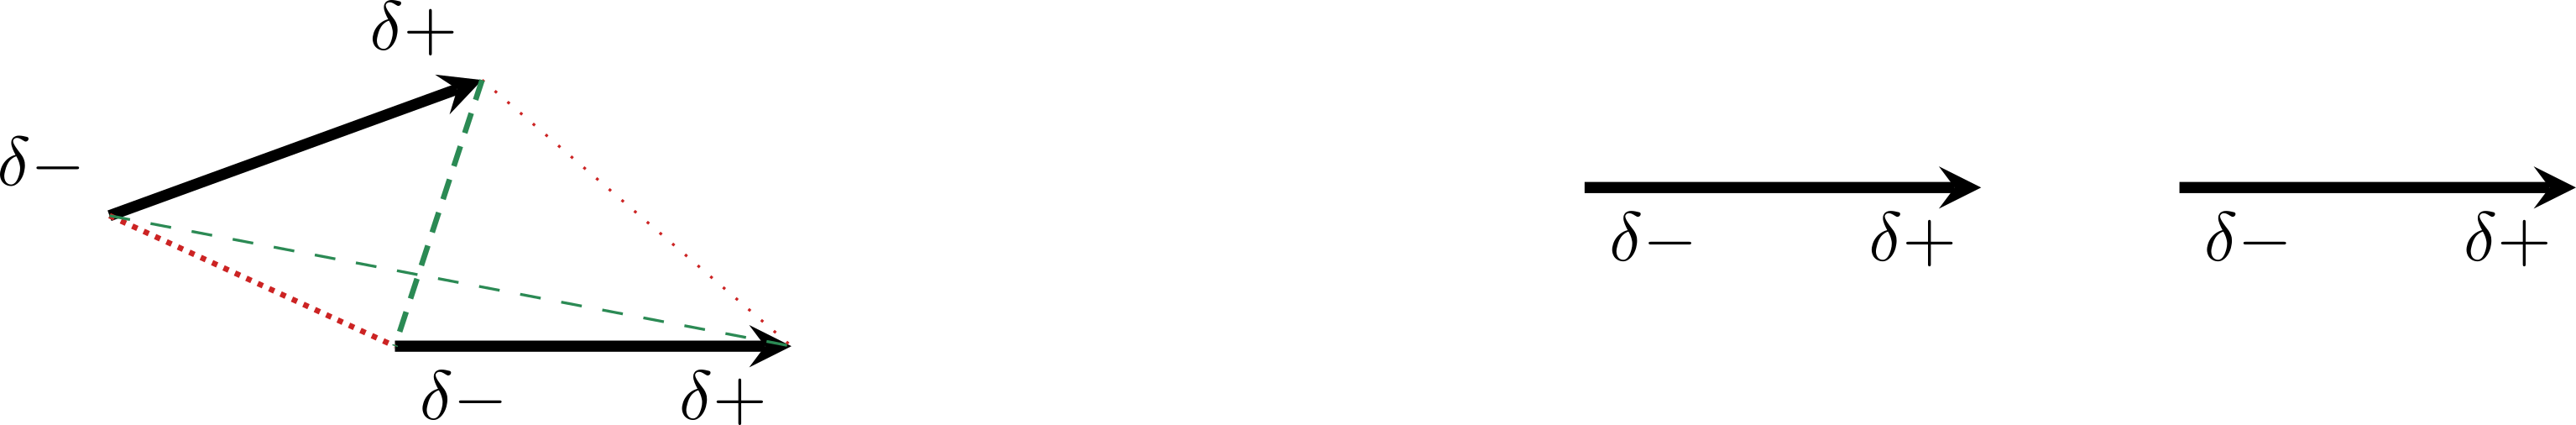
\includegraphics[scale=1]{keesom}
	}
	\caption{Interaction de \textsc{Keesom} entre deux dipôles permanents}
	\label{fig:keesom}
\end{figure}

Ce mécanisme d'interaction entre deux dipôles permanents définit l'interaction
de \textsc{Keesom,} qui fait partie des interactions de \textsc{Van der Waals}.
On peut résumer ses propriétés~:
\begin{tcb*}[breakable](defi){Interaction de \textsc{Keesom}}
	\begin{itemize}[label=$\diamond$]
		\bitem{Nature}~: \psw{
			force entre 2 molécules polaires (dipôle permanent/dipôle permanent).
		}
		\bitem{Énergie potentielle}~:
		\psw{
			\[\Ec_p = -k \frac{\mu_{\ce{A}}{}^2\mu_{\ce{B}}{}^2}{d^6}\]
		}
		avec $\mu_{\ce{A}}$ et $\mu_{\ce{B}}$ les moments dipolaires de A et B, $k$
		une constante physique (dépendant de $T$).
		\bitem{Énergie de liaison}~:
		\psw{
			\SIrange{0.5}{3}{kJ.mol^{-1}}
		}
	\end{itemize}
	Cette interaction est assez faible car elle dépend de l'orientation des dipôles.
\end{tcb*}


L'énergie d'une liaison de correspond à l'énergie nécessaire pour pour casser
\SI{1}{mol} de liaisons.

\subsection{Interaction de \textsc{Debye}~: permanent/induit}

Comme introduit dans le chapitre précédent, les molécules ne sont pas des
solides mais peuvent se déformer, en particulier sous l'effet des forces de
Coulomb subies par les noyaux et les électrons. Cette capacité est traduite par
la \textbf{polarisabilité}, dont on rappelle les caractéristiques ici~:
\begin{tcb*}(rapp){Polarisabilité}
	La capacité qu'a le nuage électronique d'une molécule de se déformer est
	quantifiée par sa polarisabilité, nombre sans dimension souvent noté $\a$.
	\bigbreak
	En général, une molécule est d'autant plus polarisable qu'elle est
	«~volumineuse~», ce qui est souvent équivalent à dire que sa masse
	molaire/son numéro atomique est élevé(e).
\end{tcb*}

Ainsi, lorsqu'une molécule polaire se trouve à proximité d'une molécule
apolaire, le nuage électronique de la molécule apolaire se déforme. La
Figure~\ref{fig:debye} représente très schématiquement un exemple d'une telle
situation~: un excès de charge négative $\de'-$ se forme au voisinage de la
charge partielle $\de+$ de la molécule polaire.
\bigbreak
Finalement, la molécule
initialement apolaire acquiert à son tour un moment dipolaire $\muf\ind{ind}$~:
on parle de moment dipolaire \textbf{induit}, ou dipôle induit. Ce dipôle induit
interagit alors avec le dipôle permanent de l'autre molécule comme pour
l'interaction de \textsc{Keesom}~: cette interaction particulière est celle dite
de \textsc{Debye}.

\begin{figure}[H]
	\centering
	\sswitch{
		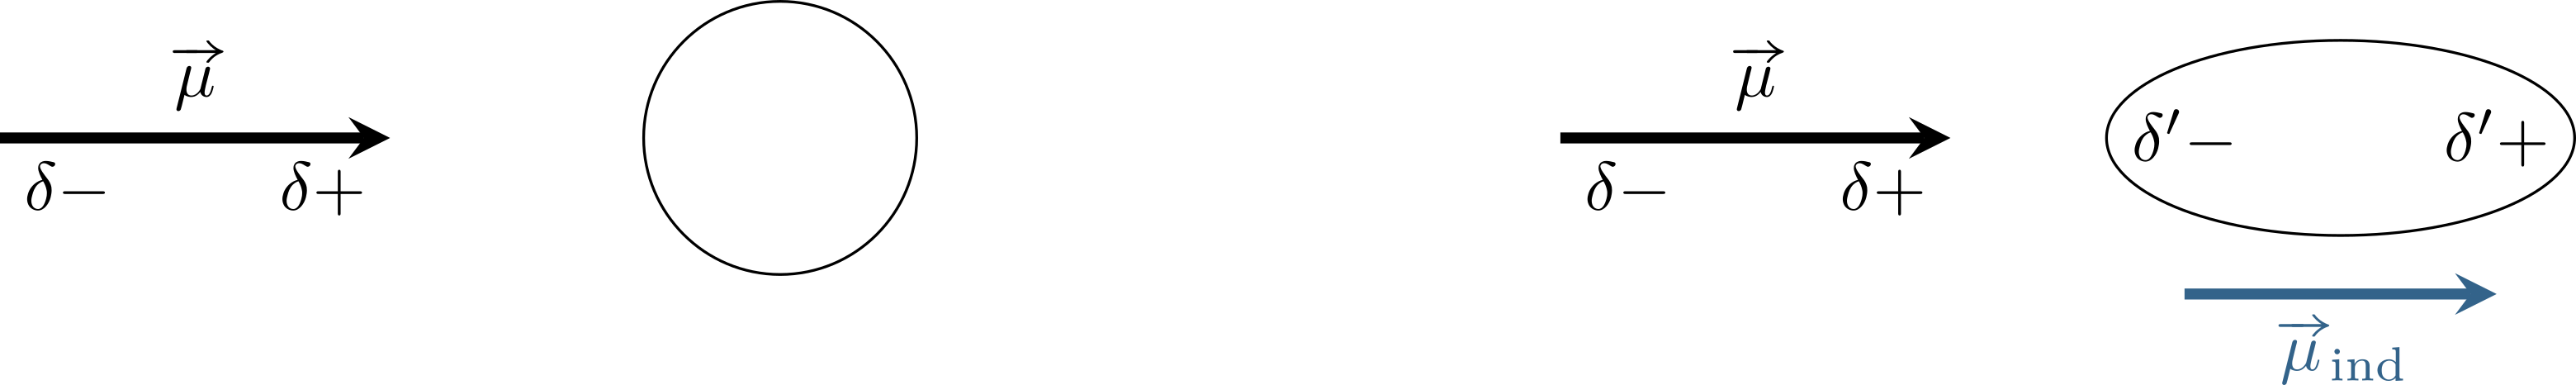
\includegraphics[scale=1, draft=true]{debye}
	}{
		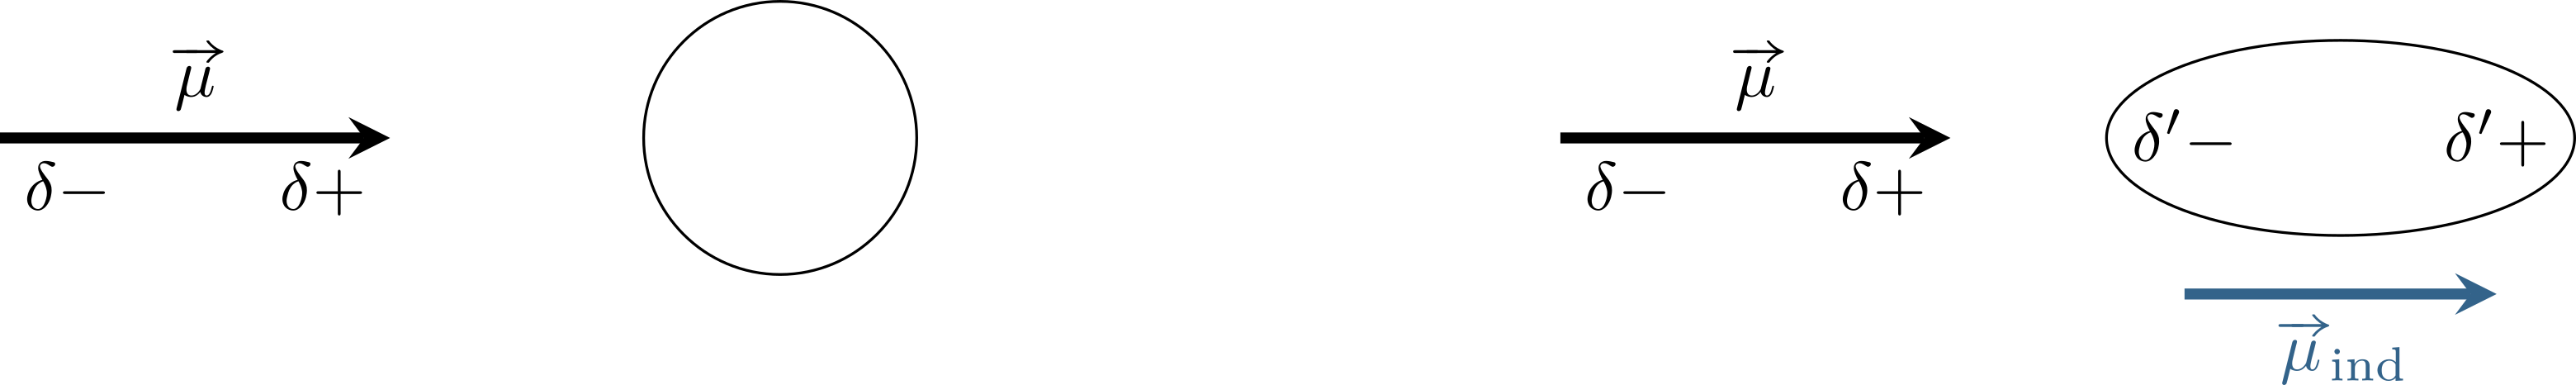
\includegraphics[scale=1]{debye}
	}
	\caption{Interaction de \textsc{Debye} entre un dipôle permanent et un
		dipôle induit.}
	\label{fig:debye}
\end{figure}

Ainsi, pour l'interaction de \textsc{Debye}~:
\begin{tcb*}(defi){Interaction de \textsc{Debye}}
	\begin{itemize}[label=$\diamond$]
		\bitem{Nature}~:
		\psw{
			force entre 1 molécule polaire et 1 apolaire (dipôle permanent/dipôle
			induit).
		}
		\bitem{Énergie potentielle}~:
		\psw{
			\[\Ec_p = -k' \frac{\mu_{\ce{A}}{}^2\a_{\ce{B}}}{d^6}\]
		}
		avec $\mu_{\ce{A}}$ le moment dipolaire de A et $\a_{\ce{B}}$ la
		polarisabilité de B, $k'$ constante (dépend de $T$).
		\bitem{Énergie de liaison}~:
		\psw{
			\SIrange{0.02}{0.5}{kJ.mol^{-1}}
		}
	\end{itemize}
	L'effet est donc en général comparable à celui des interactions de
	\textsc{Keesom}, et cette énergie sera d'autant plus grande (en valeur
	absolue) que le dipôle permanent sera grand et que la polarisabilité aussi (donc
	molécule apolaire grande).
\end{tcb*}

\subsection{Interaction de \textsc{London}~: induit/induit}

Enfin, même si elle est globalement apolaire, le mouvement incessant des
électrons fait qu'une molécule possède toujours un moment dipolaire instantané
(c'est une image~: le moment dipolaire instantané est d'origine quantique).
Comme attendu, ce moment dipolaire instantané est d'autant plus grand que la
molécule est polarisable. Ces moments dipolaires peuvent ensuite interagir entre
eux, ce qui se traduit globalement par une interaction attractive entre les
molécules, appelée interaction de \textbf{\textsc{London}}, qui fait partie des
interactions de \textsc{Van der Waals}.

\begin{tcb*}(defi){Interaction de \textsc{London}}
	\begin{itemize}[label=$\diamond$]
		\bitem{Nature}~:
		\psw{
			force entre 2 molécules apolaires (dipôle induit/dipôle induit).
		}
		\bitem{Énergie potentielle}~:
		\psw{
			\[\Ec_p = -k'' \frac{\a_{\ce{A}}\a_{\ce{B}}}{d^6}\]
		}
		avec $\a_{\ce{A}}$ et $\a_{\ce{B}}$ la polarisabilité de A et B, $k''$
		une constante physique (dépendant de $T$).
		\bitem{Énergie de liaison}~:
		\psw{
			\SIrange{0.5}{30}{kJ.mol^{-1}}
		}
	\end{itemize}
	Les interactions de \textsc{London} peuvent donc être largement dominantes sur
	les deux autres \textbf{selon les polarisabilités} mises en jeu.
\end{tcb*}

\subsection{Bilan et comparaison}

\begin{tcb*}(ror){Bilan des interactions de \textsc{Van der Waals}}
	\begin{center}
		\captionof{table}{Comparaison des propriétés des interactions de
			\textsc{Van der Waals}.}
		\label{tab:vdwcomp}
		\begin{tabular}{ccccc}
			\toprule
			Nom             & Type d'interaction    & Condition d'existence    & Nature     & Énergie de
			liaison
			\\\midrule
			\textsc{Keesom} & permanent-permanent   & molécules polaires       & attractive
			                & \SI{1}{kJ.mol^{-1}}
			\\
			\textsc{Debye}  & permanent-induit      & 1 polaire, 1 polarisable & attractive
			                & \SI{0.1}{kJ.mol^{-1}}
			\\
			\textsc{London} & induit-induit         & molécules polarisables   & attractive
			                & \SI{10}{kJ.mol^{-1}}
			\\\bottomrule
		\end{tabular}
	\end{center}
\end{tcb*}

\begin{tcb*}[breakable](rema)<lftt>{Autour des interactions}
	\begin{itemize}[label=$\diamond$]
		\item Les interactions de \textsc{Van der Waals} sont toujours attractives.
		\item L'énergie d'une liaison de \textsc{Van der Waals} est de l'ordre de
		      quelques kilojoule par mole, soit cent fois moins qu'une liaison
		      covlante~: on les qualifie de liaisons faibles.
		\item Plus une \textbf{liaison est faible}, plus la \textbf{longueur de
			      liaison est grande}~: deux molécules «~liées~» entre elles par une liaison
		      de \textsc{Van der Waals} sont malgré tout relativement éloignées l'une de
		      l'autre.
		\item Comme \textbf{toutes les molécules sont polarisables}, toutes sont
		      sujettes aux interactions de \textsc{Van der Waals}. Plus la masse molaire
		      d'une molécule est élevée, plus sa polarisabilité $\a$ augmente.
	\end{itemize}
\end{tcb*}

\begin{tcb*}(exem)<lftt>{Ordres de grandeurs d'interactions de \textsc{Van der
				Waals}}
	\begin{center}
		\captionof{table}{Contributions relatives des trois interactions de
			\textsc{VdW} à l'énergie totale.}
		\label{tab:vdwcont}
		\begin{tabular}{cccccc}
			\toprule
			\multirow{2}{*}[-3pt]{Espèce}                    &
			\multirow{2}{*}[-3pt]{Moment dipolaire (\si{D})} &
			\multirow{2}{*}[-3pt]{Polarisabilité}            &
			\multicolumn{3}{c}{Contributions relatives (\%)}
			\\\cmidrule{4-6}
			                                                 &                &                 &
			\textsc{Keesom}                                  & \textsc{Debye} & \textsc{London}
			\\\midrule
			\ce{He}                                          & 0              & \num{0.2}       & 0  & 0 & 100
			\\
			\ce{H2}                                          & 0              & \num{0.79}      & 0  & 0 & 100
			\\
			\ce{H2O}                                         & \num{1.85}     & \num{1.48}      & 69 & 7 & 24
			\\
			\ce{NH3}                                         & \num{1.47}     & \num{2.22}      & 34 & 9 & 57
			\\
			\ce{HCl}                                         & \num{1.08}     & \num{2.63}      & 9  & 5 & 86
			\\
			\ce{HBr}                                         & \num{0.79}     & \num{3.61}      & 2  & 2 & 96
			\\
			\bottomrule
		\end{tabular}
	\end{center}
\end{tcb*}

\subsection{Forces répulsives et distance des interactions}
En ne considérant que les interactions de \textsc{Van der Waals}, les molécules
devraient donc s'attirer jusqu'à $d=0$, ce qui n'est pas le cas~: la matière ne
s'effondre pas. En réalité, \textbf{il existe des forces répulsives} et qui
compensent les forces de \textbf{VdW} à très courte distance. Elles sont dues au
fait que les nuages électroniques ne peuvent s'interpénétrer. Elles sont
associées à une énergie potentielle de répulsion~:
\psw{
	\[\Ec_p = + \frac{B}{d^{12}}\]
}
d'où l'énergie potentielle totale, tracée Figure~\ref{fig:eprep}~:
\psw{
	\[
		\Ec_{p, \tot} =
		\underbracket[1pt]{-\frac{A}{d^6}}\ind{attraction}
		\underbracket[1pt]{+\frac{B}{D^{12}}}\ind{répulsion}
	\]
}

\begin{figure}[h!]
	\centering
	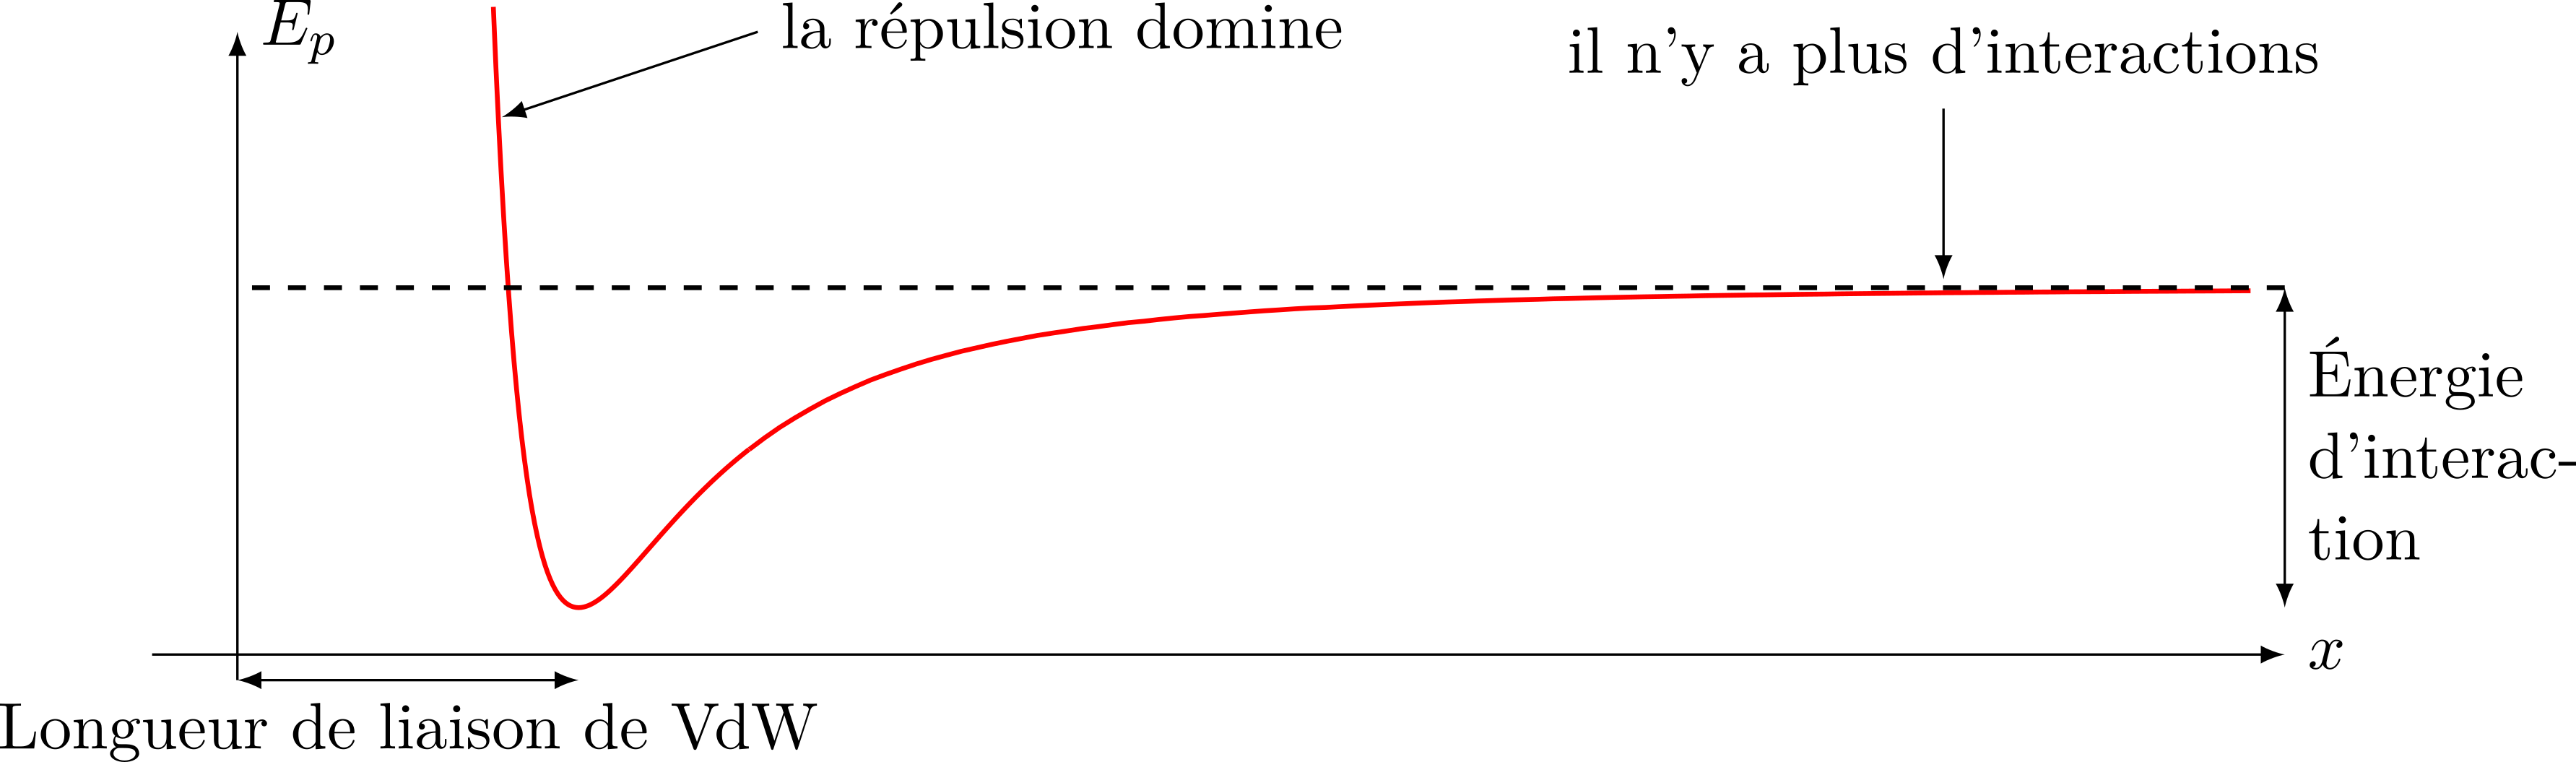
\includegraphics[scale=1]{eprep}
	\caption{Forme de l'énergie potentielle totale d'interaction entre deux
		molécules.}
	\label{fig:eprep}
\end{figure}
L'énergie totale est attractive à longue distance, mais répulsive à très courte
distance.
\begin{tcb*}[cnt](ror){Distance des liaisons de VdW}
	\psw{
		La distance d'équilibre est autour de \SIrange{300}{500}{pm}.
	}
\end{tcb*}

\section{Températures de changement d'état}
La température d'un changement d'état résulte de la compétition entre deux
énergies~:
\begin{itemize}
	\item \psw{
		      D'une part l'énergie thermique, de l'ordre de $RT$ ($\approx
			      \SI{2.5}{kJ.mol^{-1}}$ à $T\ind{ambiant}$)~;
	      }
	\item \psw{
		      D'autre part l'énergie de cohésion liée aux interactions de
		      \textsc{VdW} ($\approx \SI{1}{kJ.mol^{-1}}$).
	      }
\end{itemize}
Chauffer un composant revient à donner suffisamment d'énergie cinétique à un
atome ou molécule pour qu'elle quitte le puits de potentiel qui la relie à un
autre atome ou molécule (voir Figure~\ref{fig:eprep}). Ainsi,
\begin{tcb*}[cnt, bld](ror){Changement d'état et énergie de liaison}
	\psw{
		Plus les interactions attractives sont fortes, plus les températures de
		changement d'état sont élevées.
	}
\end{tcb*}

\subsection{Influence de la polarité}
\subsubsection{Exemple 1~: \ce{CO} et \ce{NO}}
\vspace{-10pt}
\begin{isd}
	\begin{center}
		\captionof{table}{Caractéristiques de \ce{CO} et \ce{NO}.}
		\label{tab:cono}
		\begin{tabular}{ccc}
			\toprule
			Édifice & $\mu$ (\si{D}) & $\tt\ind{eb}
				(\si{\degreeCelsius})$
			\\\midrule
			\ce{CO} & \num{0.112}    & \psw{\num{-191.5}}
			\\
			\ce{NO} & \num{0.153}    & \psw{\num{-151.8}}
			\\
			\bottomrule
		\end{tabular}
	\end{center}
	\tcblower
	\begin{itemize}
		\item \psw{
			      Même taille et éléments proches $\Ra$ même polarisabilité $\Ra$ même
			      \textsc{London}.
		      }
		\item \psw{
			      $\mu_{\ce{NO}} > \mu_{\ce{CO}} \Ra $ \textsc{Debye} et
			      \textsc{Keesom} $\nearrow$
		      }
	\end{itemize}
	\vspace{-15pt}
	\begin{gather*}
		\beforetext{D'où}
		\boxed{\psw{\tt\ind{eb,NO} > \tt\ind{eb,CO}}}
	\end{gather*}
\end{isd}

\subsubsection{Exemple 2~: isomères du 1,2-chloroéthène}
\bigbreak
\noindent
\begin{minipage}{0.29\linewidth}
	\begin{gather*}
		\cfig{
		@{Cg1}C
		(-[3]@{Clg1}Cl)
		(-[5]H)
		=_[@{mid1}0]@{Cd1}C
		(-[1]@{Cld1}Cl)
		(-[7]H)
		}
		\chemmove[\sswitch{white}{red}, -stealth]{
			\draw
			(mid1) --++
			(0,-40pt)
			node [right] {$\muf$};
			\draw[transform canvas={xshift=4pt, yshift=4pt}, -stealth]
			(Clg1) --
			node [midway, above, sloped] {$\muf_{\ce{CCl}}$}
			(Cl1);
			\draw[transform canvas={xshift=-4pt, yshift=4pt}, -stealth]
			(Cld1) --
			node [midway, above, sloped] {$\muf_{\ce{CCl}}$}
			(Cl1);
		}
		\\
		\text{(Z)-1,2-dichloroéthène}
		\\
		\tt\ind{eb} = \psw{\SI{60}{\degreeCelsius}}
	\end{gather*}
\end{minipage}
\hfill
\begin{minipage}{0.70\linewidth}
	\begin{isd}[righthand ratio=.60]
		\begin{gather*}
			\cfig{
			@{Cg2}C
			(-[3]H)
			(-[5]@{Clg2}Cl)
			=_[@{mid2}0]@{Cd2}C
			(-[1]@{Cld2}Cl)
			(-[7]H)
			}
			\chemmove[\sswitch{white}{red}, -stealth]{
				\node[below] at (mid2) {$\muf = \of$};
				\draw[transform canvas={xshift=-4pt, yshift=2pt}, -stealth]
				(Clg2) --
				node [midway, above, sloped] {$\muf_{\ce{CCl}}$}
				(Cg2);
				\draw[transform canvas={xshift=-4pt, yshift=4pt}, -stealth]
				(Cld2) --
				node [midway, above, sloped] {$\muf_{\ce{CCl}}$}
				(Cd2);
			}
			\\
			\text{(E)-1,2-dichloroéthène}
			\\
			\tt\ind{eb} = \psw{\SI{48}{\degreeCelsius}}
		\end{gather*}
		\tcblower
		\begin{itemize}
			\item \psw{
				      Même taille $\Ra$ même $\alpha$ $\Ra$ même \textsc{London}
			      }
			\item \psw{
				      $\mu\ind{Z} > \mu\ind{E} \Ra$ \textsc{Debye} et \textsc{Keesom}
				      $\nearrow$
			      }
		\end{itemize}
		\vspace{-15pt}
		\begin{gather*}
			\beforetext{D'où}
			\boxed{\psw{\tt\ind{eb,Z} > \tt\ind{eb,E}}}
		\end{gather*}
	\end{isd}
\end{minipage}

\subsubsection{Conclusion}
On observe ici~:
\begin{tcb*}(ror){Température changement d'état et moment dipolaire}
	\psw{
		Plus le \textbf{moment dipolaire est grand}, plus les espèces ont une forte
		cohésion, et donc plus la \textbf{température} de changement d'état est
		\textbf{élevée} (à polarisabilité proche).
	}
\end{tcb*}

\subsection{Influence de la polarisabilité}
\subsubsection{Exemple 1~: composés hydrogénés de la 14\ieme\ colonne}
\smallbreak
\noindent
\begin{isd}[lefthand ratio=.45]
	\begin{center}
		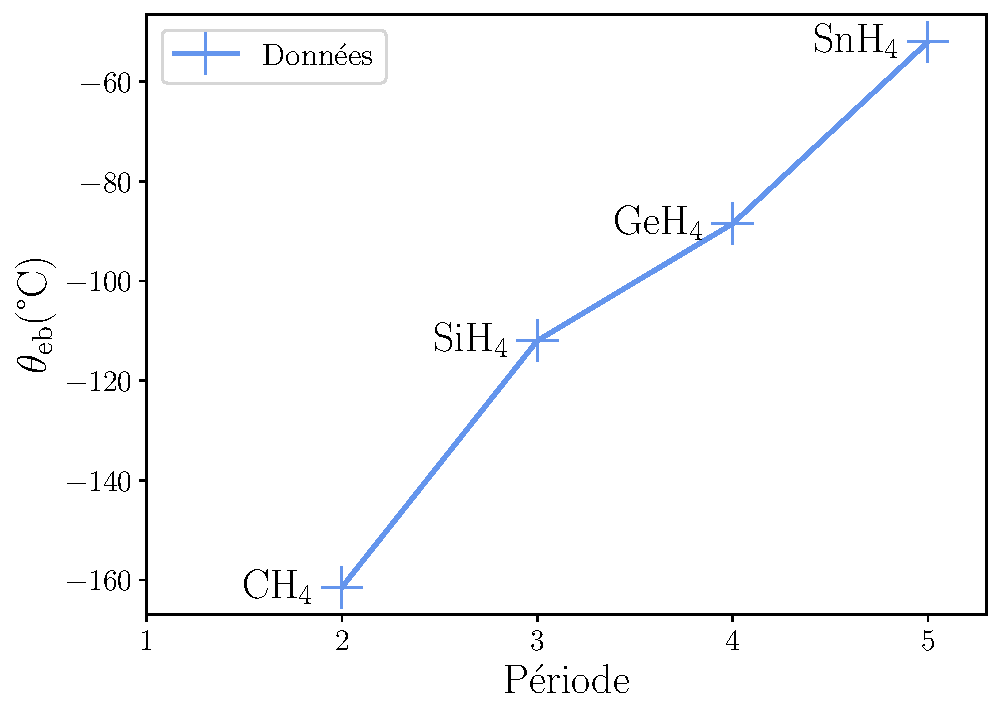
\includegraphics[width=\linewidth]{hydro_14}
		\captionsetup{justification=centering}
		\captionof{figure}{Évolution des $\tt\ind{eb}$ des composés hydrogénés de la
			famille du carbone.}
	\end{center}
	\tcblower
	\begin{itemize}
		\item \psw{
			      Molécules pratiquement apolaires (géométrie AX$_4$ symétrique)
			      $\Ra$ peu de \textsc{Debye} et \textsc{Keesom}~;
		      }
		\item \psw{
			      $\alpha \nearrow \text{~avec~} n
				      \Ra \textsc{London} \nearrow \text{~avec~} n$
		      }
	\end{itemize}
	\vspace{-15pt}
	\begin{gather*}
		\beforetext{Ainsi}
		\boxed{\psw{T\ind{eb} \nearrow \text{~avec~} n}}
	\end{gather*}
\end{isd}

\subsubsection{Exemple 2~: dihalogènes}
\begin{isd}
	\begin{center}
		\captionsetup{justification=centering}
		\captionof{table}{Températures de changement d'état pour des dihalogènes.}
		\label{tab:dihaltemp}
		\begin{tabular}{ccc}
			\toprule
			Édifice  & $\tt\ind{fus} (\si{\degreeCelsius})$ & $\tt\ind{eb}
				(\si{\degreeCelsius})$
			\\\midrule
			\ce{Cl2} & \num{-102}                           & \num{-34}
			\\
			\ce{Br2} & \num{-7}                             & \num{59}
			\\
			\ce{I2}  & \num{113}                            & \num{185}
			\\
			\bottomrule
		\end{tabular}
	\end{center}
	\tcblower
	\begin{itemize}
		\item \psw{
			      Molécules apolaires
			      $\Ra$ pas de \textsc{Debye} et \textsc{Keesom}~;
		      }
		\item \psw{
			      $\alpha \nearrow \text{~avec~} n
				      \Ra \textsc{London} \nearrow \text{~avec~} n$
		      }
	\end{itemize}
	\vspace{-15pt}
	\begin{gather*}
		\beforetext{Ainsi}
		\boxed{\psw{T\ind{eb} \nearrow \text{~avec~} n}}
	\end{gather*}
\end{isd}

\subsubsection{Conclusion}
\begin{tcb*}(ror){Température changement d'état et polarisabitié}
	\psw{
		Plus une molécule est \textbf{polarisable}, c'est-à-dire grande en taille,
		plus les températures de changement d'état sont \textbf{élevées}.
	}
\end{tcb*}

\section{Liaison hydrogène}
\subsection{Introduction}
La polarisabilité décroît notablement lorsque l'on remonte une colonne du
tableau périodique~; ainsi, en considérant les interactions de \textsc{Van der
	Waals}, on s'attend à ce que~:
\begin{tasks}(3)
	\task \ce{NH3} bouille à $\approx \SI{-130}{\degreeCelsius}$~;
	\task \ce{HF} bouille à $\approx \SI{-120}{\degreeCelsius}$.
	\task \ce{H2O} bouille à $\approx \SI{-80}{\degreeCelsius}$~;
\end{tasks}
Or, ça n'est évidemment pas le cas.

\noindent
\begin{minipage}[t]{0.45\linewidth}
	\vspace{0pt}
	\begin{center}
		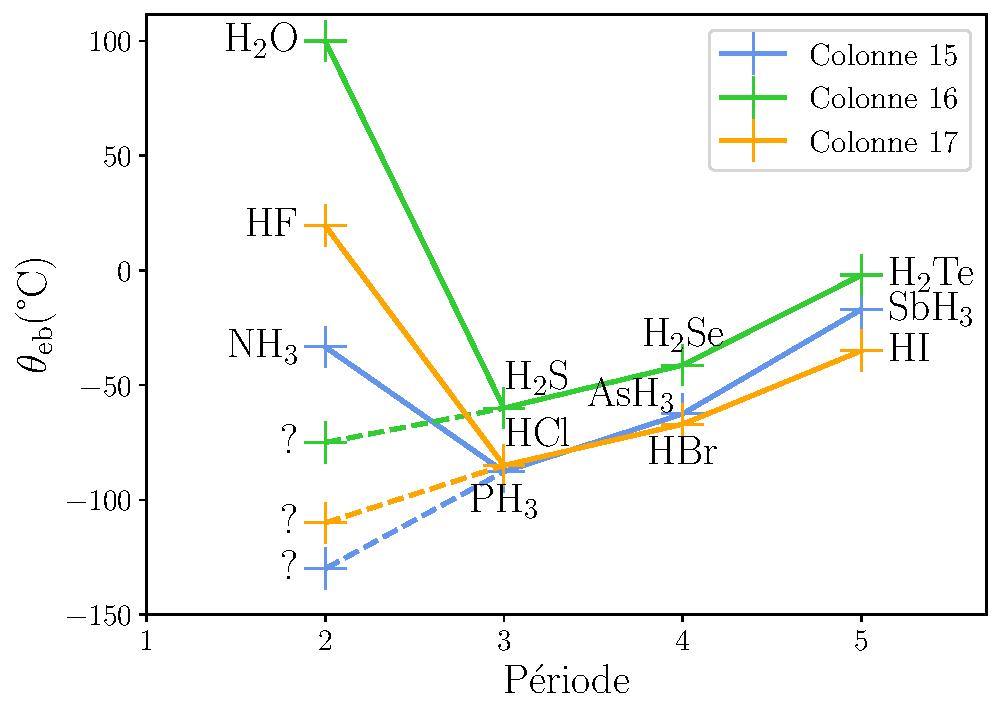
\includegraphics[width=\linewidth]{LH}
		% \captionsetup{justification=centering}
		\captionof{figure}{Températures d'ébullition des composés hydrogénés des
			colonnes 15 à 17. En pointillé les températures attendues en considérant
			les interactions de \textsc{VdW} uniquement. Les températures observées
			sont en traits pleins, et s'expliquent par l'existence de la liaison
			hydrogène.}
	\end{center}
\end{minipage}
\hfill
\begin{minipage}[t]{0.50\linewidth}
	\vspace{0pt}
	\begin{center}
		\begin{threeparttable}
			\captionsetup{justification=centering}
			\captionof{table}{Comparaison des propriétés du chloroéthane et de
				l'éthanol.}
			\label{tab:chlocomp}
			\begin{tabular}{lccc}
				\toprule
				Nom          & Représentation & $\mu$ (\si{D}) & $\tt\ind{eb}
					(\si{\degreeCelsius})$
				\\\midrule
				Chloroéthane &
				\cfig{[,.5]
				C
				(-[2]\lewis{024,Cl})
				(-[4]H)
				(-[6]H)
				-C
				(-[0]H)
				(-[2]H)
				(-[6]H)
				}            &
				\num{2.06}   & \num{12}
				\\\midrule
				Éthanol      &
				\cfig{[,.5]
				C
				(-[2]H)
				(-[4]H)
				(-[6]H)
				-C
				(-[2]H)
				(-[6]H)
				-\lewis{26,O}
				-H
				}            &
				\num{1.71}   & \num{60}
				\\\bottomrule
			\end{tabular}
			\begin{tablenotes}[flushleft]
				\small
				\item \textbf{Observation.} En dépit d'une polarisabilité
				\textbf{et} d'un moment dipolaire plus faible, l'éhanol a une plus
				grande cohésion que le chloroéthane.
			\end{tablenotes}
		\end{threeparttable}
	\end{center}
\end{minipage}

\subsection{Définition et exemples}
\begin{tcb*}(defi){Liaison hydrogène}
	Une \textbf{liaison hydrogène} s'établit entre un atome d'\textbf{hydrogène
		porté par un atome très électronégatif} (\ce{N}, \ce{O} ou \ce{F}) et un autre
	atome \ce{B} également très électronégatif, porteur d'au moins un
	\textbf{doublet non-liant} et neutre.
	\bigbreak
	Autrement dit, la liaison hydrogène se fait entre un hydrogène dans une
	liaison ionisée et un doublet non-liant d'un atome électronégatif. Elle se
	représente par un trait pointillé.
	\psw{
		\begin{center}
			\cfig{
				\lewis{24,O}
				(-[6,.7]H)
				(-[0,.7]@{hg}H)
			}
			\hspace{1.5cm}
			\cfig{
				@{Oh}\lewis{24,O}
				(-[6,.7]H)
				(-[0,.7]H)
			}
			\chemmove[dashed, -]{
				\draw
				([shift={(2pt,0)}]hg.east) --
				node [midway, above]
				{\scriptsize Liaison}
				node [midway, below]
				{\scriptsize hydrogène}
				([shift={(-4pt,0)}]Oh.west)
				;}
		\end{center}
	}
\end{tcb*}

\begin{tcb*}(ror){Caractéristiques de la LH}
	L'énergie d'une liaison hydrogène est de l'ordre de quelques dizaines de
	\si{kJ.mol^{-1}}, soit dix fois plus qu'une liaison de \textsc{Van der
		Waals} typique et dix fois moins qu'une liaison covalente.
	\psw{
	\[
		\underbracket[1pt]{E\ind{covalente}}_{\approx\SI{500}{kJ.mol^{-1}}}
		\gg
		\underbracket[1pt]{E\ind{LH}}_{\approx\SI{20}{kJ.mol^{-1}}}
		\gg
		\underbracket[1pt]{E\ind{VdW}}_{\approx\SI{1}{kJ.mol^{-1}}}
	\]
	}
	Une liaison hydrogène est environ deux fois plus longue qu'une liaison
	covalente~:
	\psw{
		\[
			\underbracket[1pt]{\ell\ind{covalente}}_{\approx\SI{100}{pm}}
			\ll
			\underbracket[1pt]{\ell\ind{LH}}_{\approx\SI{200}{pm}}
			\ll
			\underbracket[1pt]{\ell\ind{VdW}}_{\approx\SI{400}{pm}}
		\]
	}
	\vspace{-15pt}
\end{tcb*}

\begin{tcb*}(exem)<lftt>'l'{Implications de la LH}
	\begin{center}
		$\vcenter{\hbox{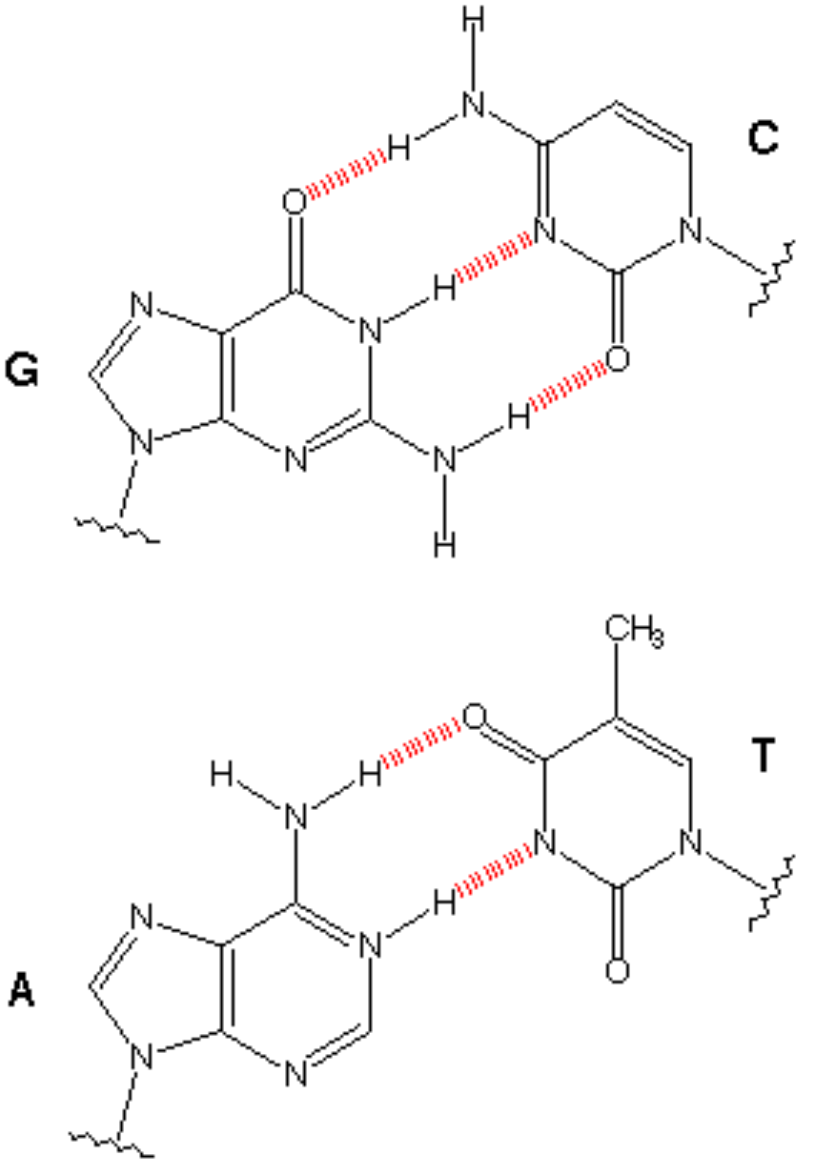
\includegraphics[scale=1]{lhex_a}}}$
		$\vcenter{\hbox{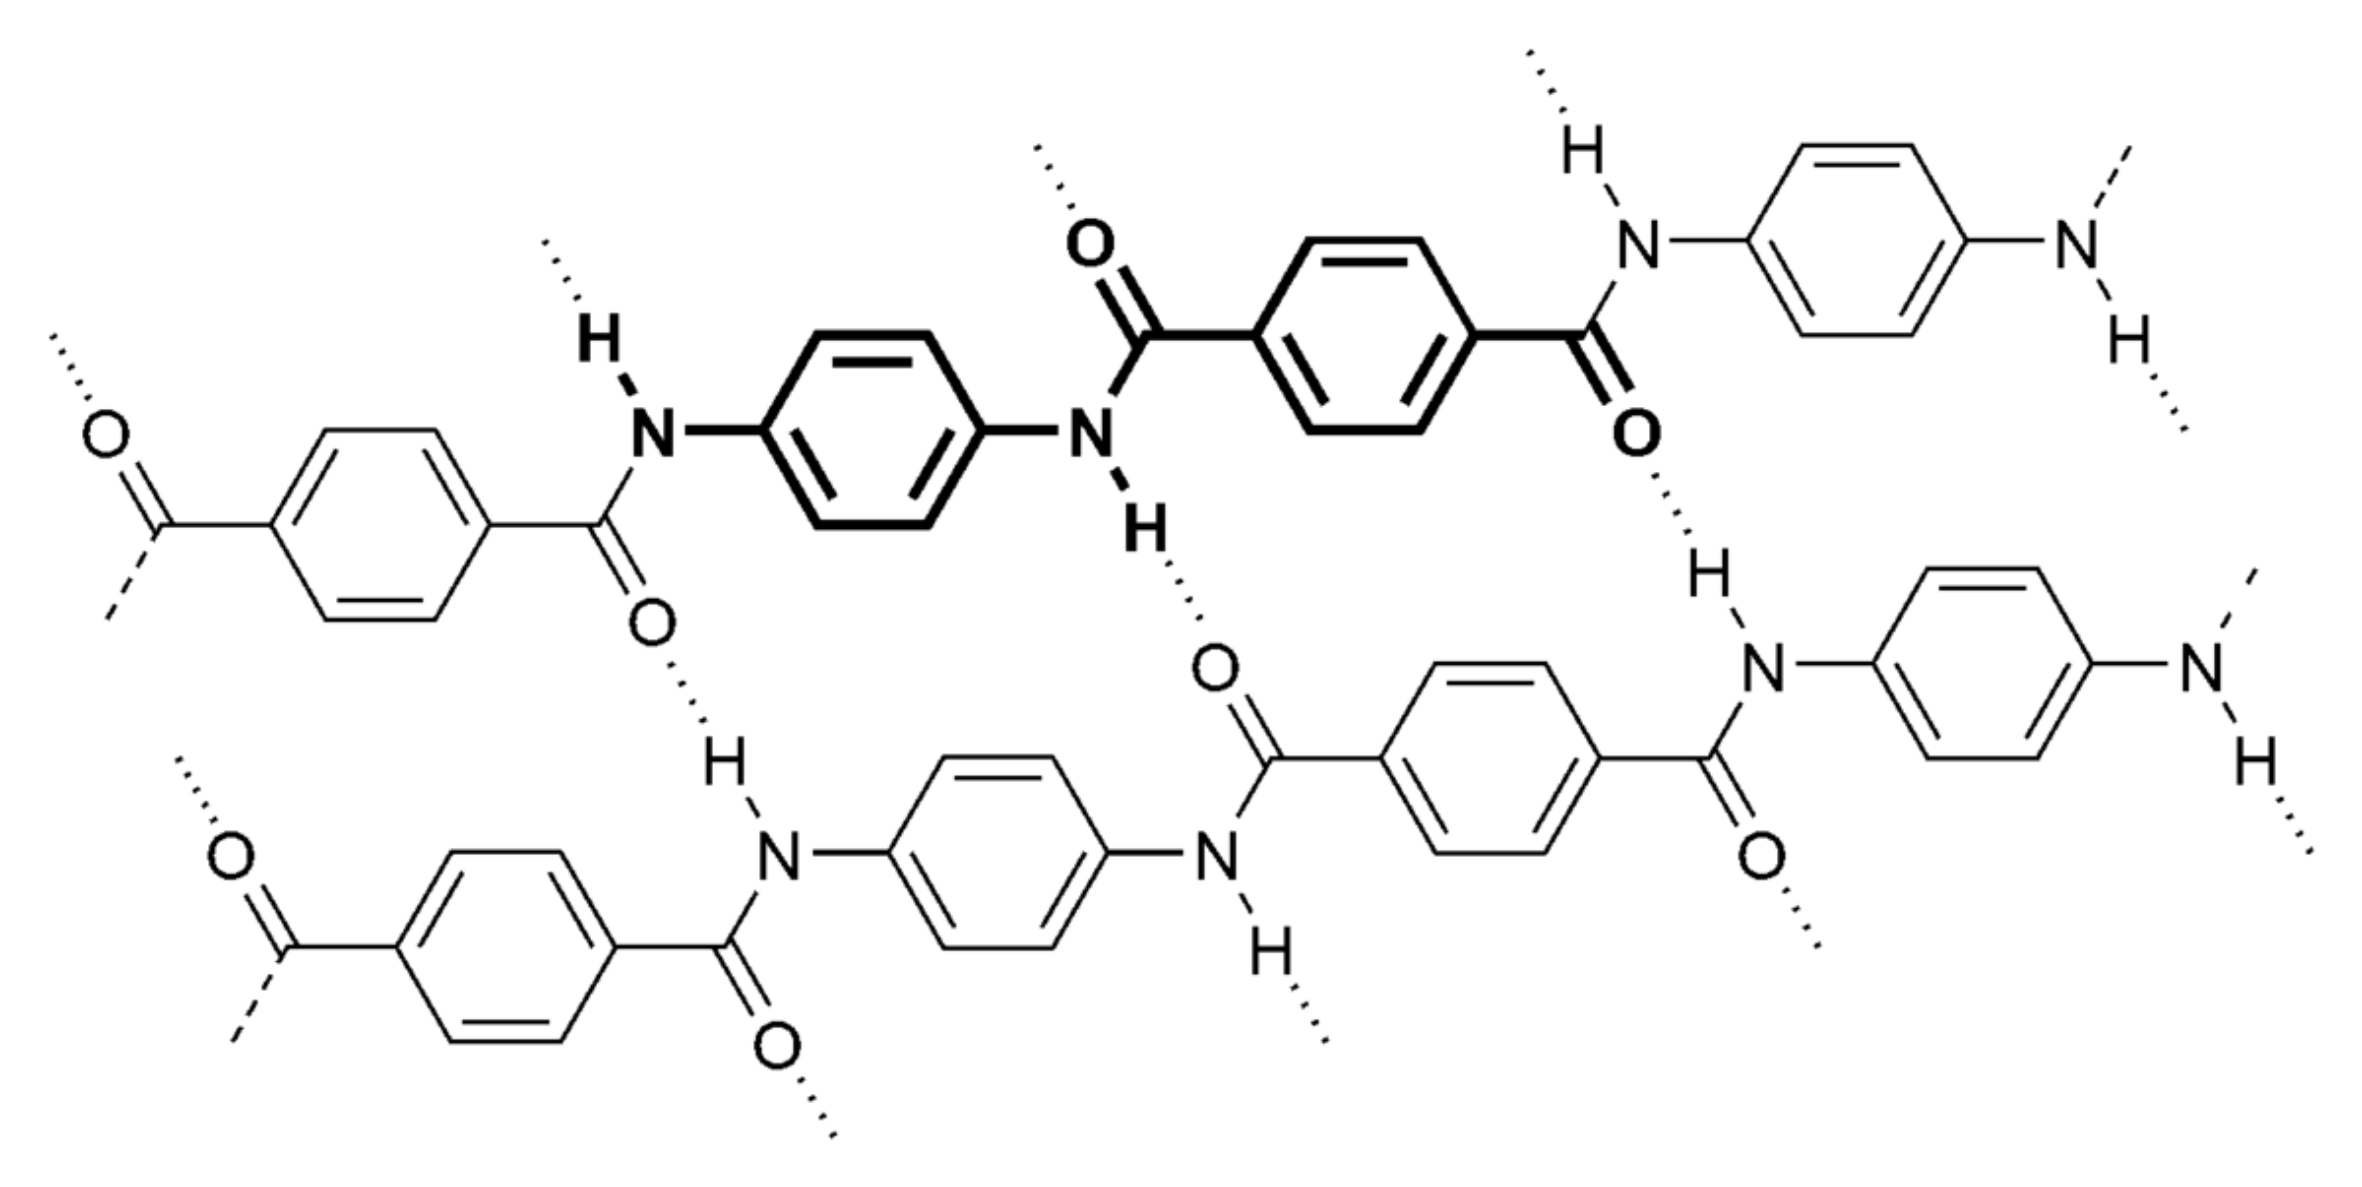
\includegraphics[scale=1]{lhex_b}}}$
	\end{center}
	\begin{itemize}
		\item Les LH expliquent la cohésion dans la double hélice de l'ADN,
		      \textit{via} la correspondance entre adénine et thymine d'une
		      part, et entre guanine et cytosine d'autre part.
		\item Les LH expliquent la cohésion entre les fibres de Kevlar.
		\item Les LH expliquent la haute température d'ébullition de nombreux
		      composés chimiques, notamment celle de l'eau.
	\end{itemize}
\end{tcb*}

\section{Solvants}
Une autre propriété macroscopique que l'on expérimente tous les jours à tous les
égards est celle des solvants, qui composent la quasi-totalité de nos
interactions physico-chimiques au quotidien. Voyons comment caractériser ces
solvants, et surtout pourquoi l'eau permet autant de réactions chimiques.

\subsection{Classement}
Les solvants sont classés selon 3 caractéristiques~:
\begin{enumerate}
	\item \psw{
		      Leur caractère \textbf{polaire ou apolaire}~;
	      }
	\item \psw{
		      Leur caractère \textbf{protique ou aprotique} (capable de
		      liaisons hydrogène ou pas)~;
	      }
	\item \psw{
		      Leur \textbf{pouvoir dispersant}.
	      }
\end{enumerate}

On a déjà parlé des 2 premières, présentons la troisième~:
\subsubsection{Pouvoir dispersant}
Lorsque deux ions de charges opposées $\pm q$ sont séparés d'une distance $d$
dans le vide, ils exercent l'un sur l'autre une force attractive de norme
\[F_0 = \frac{q^2}{4\pi\ep_0d^2}\]
avec $\ep_0$ la permittivité diélectrique du vide. Dans un milieu \textbf{autre
	que le vide}, par exemple un \textbf{solvant}, la force reste attractive mais le
milieu modifie la norme de cette force \textit{via} sa permittivité relative
$\ep_r$~:
\psw{
	\[F\ind{milieu} = \frac{q^2}{4\pi\ep_0\ep_rd^2} = F_0\times \frac{1}{\ep_r}\]
}

Autrement dit, quand un solvant s'infiltre \textbf{entre deux ions}, le milieu
entre les deux change et ils sont \textbf{moins attirés entre eux}.

\begin{tcb*}(defi){Permittivité relative et caractère dispersant}
	La \textbf{permittivité relative} d'un solvant est une constante, notée
	$\ep_r\footnote{Cette grandeur est reliée à l'indice optique d'un milieu~:
			on a $n=\sqrt{\ep_r}$.}$
	avec $\ep_r > 1$, caractérisant sa capacité à séparer deux ions.
	Plus elle est grande, plus il est \textbf{dispersant}, c'est-à-dire capable
	de séparer des charges. On a~:
	\begin{tasks}(3)
		\task \psw{
			$01 < \ep_r < 20$\\$\Ra$ peu dispersant~;
		}
		\task \psw{
			$20 < \ep_r < 40$\\$\Ra$ dispersant~;
		}
		\task \psw{
			$40 < \ep_r \lesssim 100$\\$\Ra$ très dispersant.
		}
	\end{tasks}
	On dit que l'interaction entre les ions est \textit{écrantée} par le solvant.
\end{tcb*}

\subsubsection{Exemple de solvants}
\vspace{-15pt}
\begin{table}[h!]
	\centering
	\begin{threeparttable}
		\caption{Exemples de solvants polaires et apolaires.}
		\label{tab:solpoapo}
		\begin{tabular}{cccccc}
			\toprule
			Solvant          & Eau\tnote{1} & Méthanol & Ammoniac & Propanone\tnote{2} &
			Cyclohexane
			\\\midrule
			\textsc{Lewis}   &
			$\vcenter{\hbox{
						\cfig{[,.7]\lewis{13,O}(-[5]H)(-[7]H)}
			}}$              &
			$\vcenter{\hbox{
				\cfig{CH_3-[,.7]\lewis{26,O}-[,.7]H}
			}}$              &
			$\vcenter{\hbox{
						\cfig{\lewis{2,N}(<:[5]H)(<[6]H)(-[7]H)}
			}}$              &
			$\vcenter{\hbox{
				\cfig{[,.7]
				C
				(=[2]\lewis{13,O})
				(-[:-20]CH_3)
				(-[:200]CH_3)
				}}}$
			                 &
			$\vcenter{\hbox{\chemfig{[,.7]
				H_2C*6(-CH_2-CH_2-CH_2-CH_2-H_2C-[,,2])
				}}}$
			\\\midrule
			Polarité         &
			\psw{Polaire}    &
			\psw{Polaire}    &
			\psw{Polaire}    &
			\psw{Polaire}    &
			\psw{Apolaire}
			\\
			$\mu$ (\si{D})   &
			\psw{\num{1.85}} &
			\psw{\num{1.65}} &
			\psw{\num{1.30}} &
			\psw{\num{2.77}} &
			\psw{0}
			\\\midrule
			Proticité        &
			\psw{Protique}   &
			\psw{Protique}   &
			\psw{Protique}   &
			\psw{Aprotique}  &
			\psw{Aprotique}
			\\\midrule
			$\ep_r$          &
			\num{78.5}       &
			\num{32.6}       &
			\num{25.0}       &
			\num{20.7}       &
			\num{2.1}
			\\
			Dispersant       &
			\psw{Fortement}  &
			\psw{Oui}        &
			\psw{Oui}        &
			\psw{Oui}        &
			\psw{Presque pas}
			\\\bottomrule
		\end{tabular}
		\begin{tablenotes}[flushleft]
			\item[1] L'eau est, pour toutes ces caractéristiques, l'un des meilleurs
			solvants sur Terre.
			\item[2] Communément appelé acétone.
		\end{tablenotes}
	\end{threeparttable}
\end{table}

\subsection{Solubilité, miscibilité}
\subsubsection{Définition}
\begin{tcb*}[sidebyside](defi){Solubilité et miscibilité}
	\tcbsubtitle{\fatbox{\textbf{Solubilité}}}
	\psw{
		La solubilité d'un \textbf{solide}, appelé soluté, est la \textbf{quantité
			maximale} qu'il est possible de \textbf{dissoudre} dans un litre de
		solution d'un solvant. Elle s'exprime en \si{g.L^{-1}} ou en
		\si{mol.L^{-1}}.
	}
	\tcblower
	\tcbsubtitle{\fatbox{\textbf{Miscibilité}}}
	\psw{
		On parle de miscibilité pour caractériser la capacité de \textbf{deux
			liquides} à se \textbf{mélanger} pour former une solution homogène.
	}
\end{tcb*}

\subsubsection{Mise en solution d'espèces ioniques}
Dans l'eau, les solides ioniques se dissolvent en trois étapes\footnote{L'étape
	d'ionisation nécessite un solvant \textbf{très polaire}.}~:
\[
	\ce{
	HCl\sol{}
	->T[(ionisation)]
	H^{+}Cl^{-}\sol{}
	->T[dissociation]
	(H+ + Cl^{-})\aqu{}
	->T[solvatation]
	H^{+}\aqu{} + Cl^{-}\aqu{}
	}\]
\begin{itemize}
	\bitem{Ionisation}~: \psw{
		lorsque la molécule de solvant possède un moment dipolaire permanent, elle
		peut ioniser les éléments~;
	}
	\bitem{Dissociation}~:
	\psw{
		le solvant affaiblit les interactions à l'intérieur du soluté pur. Cette
		étape est reliée à la \textbf{permittivité} du solvant.
	}
	\bitem{Solvatation}~:
	\psw{
		le solvant augmente ses interactions avec le soluté. La qualité dépend de
		leurs \textbf{polarités} et de leurs \textbf{proticités}.
	}
\end{itemize}
\begin{figure}[htbp!]
	\centering
	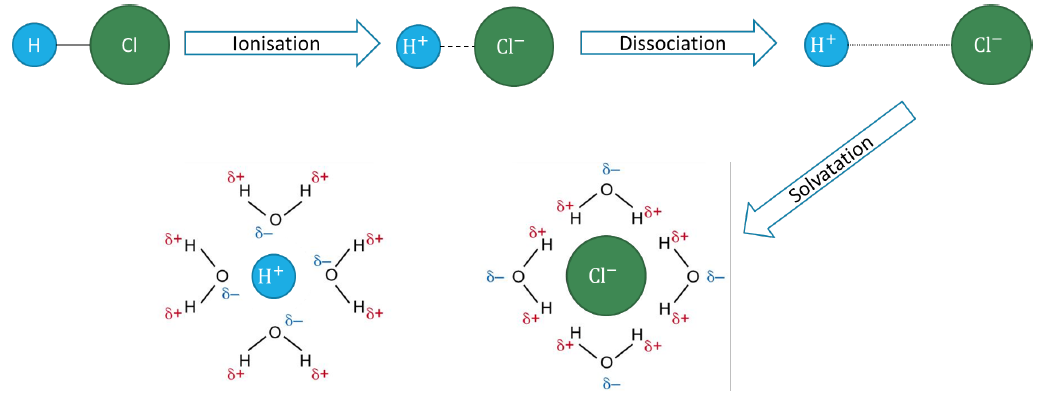
\includegraphics[width=.7\linewidth]{HCl_eau}
	\caption{Schéma du processus de solvatation de \ce{HCl} dans l’eau}
	\label{fig:hcl_eau}
\end{figure}

Notamment, si les caractéristiques du soluté et du solvant sont similaires, il
suffit de peu d'énergie/température pour que le processus se passe. Il y a de
nombreuses vidéos en
ligne\footnote{\url{https://www.youtube.com/watch?v=xdedxfhcpWo}}. Ainsi,

\begin{tcb*}[sidebyside, righthand ratio=.4](ror){Choisir un solvant}
	\begin{itemize}
		\item
		      \psw{
			      Un solvant dissout des composés semblables~;
		      }
		\item
		      \psw{
			      Deux solvants semblables sont miscibles.
		      }
	\end{itemize}
	\tcblower
	\begin{center}
		\begin{bfseries}
			\fbox{\psw{Qui se ressemble s'assemble~!}}
		\end{bfseries}
	\end{center}
\end{tcb*}

\begin{tcb*}(exem)<lftt>'l'{Solvants}
	\begin{itemize}
		\item Le glucose est très soluble dans l'eau~: \SI{700}{g.L^{-1}} à
		      $T\ind{amb}$. Il est en effet protique comme l'eau et réalise de
		      nombreuses liaisons hydrogènes.
		\item Le diiode est apolaire, il est donc peu soluble dans l'eau, mais
		      il l'est en revanche dans le cyclohexane.
		\item L'eau est un des meilleurs solvants en combinant ses propriétés
	\end{itemize}
	\begin{center}
		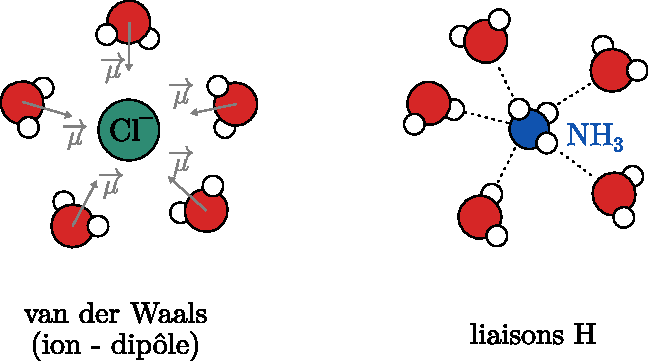
\includegraphics[width=.6\linewidth]{sol_eau}
		\captionof{figure}{Solvatation de \ce{Cl-} et \ce{NH3} par l'eau}
	\end{center}
\end{tcb*}

\end{document}
